\section{Attività di verifica}
Si analizzano qui le metriche:
\begin{itemize}
    \item \hyperref[s:mpc02]{\textbf{MPC02}}\textbf{}: \textit{Budget Variance}.
    \item \hyperref[s:mpc04]{\textbf{MPC04}}\textbf{}: \textit{Budgeted Cost of Work Scheduled}.
    \item \hyperref[s:mpc06]{\textbf{MPC06}}\textbf{}: \textit{Actual Cost of Work Performed}.
    \item \hyperref[s:mpd1]{\textbf{MPD1}}\textbf{}: Indice di Gulpease.
\end{itemize}

\subsection{MPC02 - Budget Variance}
\label{s:mpc02}
Il valore negativo riportato in Figura \ref{fig:mpc02} indica che il costo effettivo è superiore al \textit{budget} pianificato.
Il valore riportato rientra nel margine di accettabilità stabilito. \\
Il gruppo ritiene che lo sforamento del \textit{budget} sia dovuto alla generale inesperienza dei vari membri nella gestione di un progetto e nell'uso delle tecnologie, che ha portato alla necessità di incrementare il tempo di lavoro.

\begin{figure}[htbp]
    \centering
    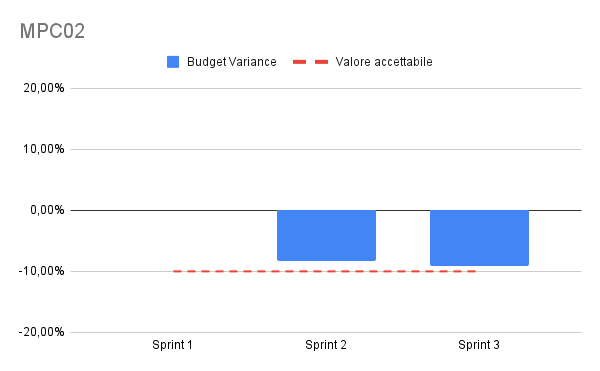
\includegraphics[width=0.7\textwidth]{img/MPC02.png}
    \caption{MPC02 - Budget Variance}
    \label{fig:mpc02}
\end{figure}


\newpage
\subsection{MPC04 - Budgeted Cost of Work Scheduled}
\label{s:mpc04}

Nel grafico in Figura \ref{fig:mpc04} è stato inserito anche il costo relativo ad ogni \textit{sprint} al fine di indicare più intuitivamente il contributo di ogni singolo \textit{sprint} al costo complessivo.\\
Il minor costo associato al quarto \textit{sprint} deriva dalla necessità di ridurre le ore di lavoro utile in concomitanza dei numerosi impegni, sia personali che legati alla sessione di esami, dei membri del gruppo.\\
Il consumo di risorse, confrontato con il preventivo dei costi presente nel documento \href{https://project-swenergy.github.io/Candidatura/Presentazione%20costi%20e%20assunzione%20impegni.pdf}{Presentazione costi ed assunzione impegni v2.0.0}, risulta ragionevole in considerazione della diversa durata delle fasi RTB e PB.
\begin{figure}[htbp]
    \centering
    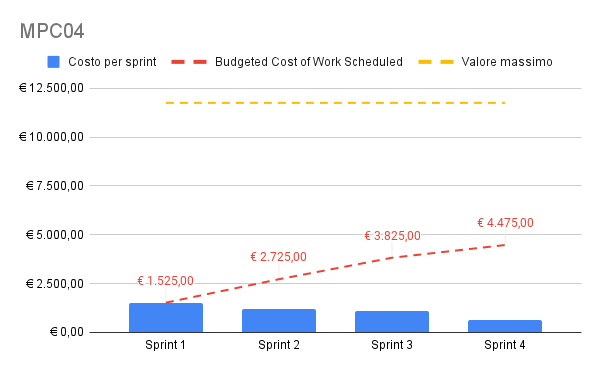
\includegraphics[width=0.7\textwidth]{img/MPC04.png}
    \caption{MPC04 - Budgeted Cost of Work Scheduled}
    \label{fig:mpc04}
\end{figure}

\subsection{MPC06 - Actual Cost of Work Performed}
\label{s:mpc06}
Il valore riportato in Figura \ref{fig:mpc06} indica che, a seguito del primo \textit{sprint}, il costo effettivo sostenuto ha superato quello preventivato.\\
Il gruppo ritiene che che il superamento del costo preventivato sia dovuto alla generale inesperienza dei vari membri nella gestione di un progetto e nell'uso delle tecnologie, che ha portato alla necessità di incrementare il tempo di lavoro nella fase iniziale del progetto.\\
Nonostante il superamento del valore ottimale, il costo effettivo è rimasto complessivamente all'interno del margine di accettabilità indicato nella metrica in esame.

\begin{figure}[htbp]
    \centering
    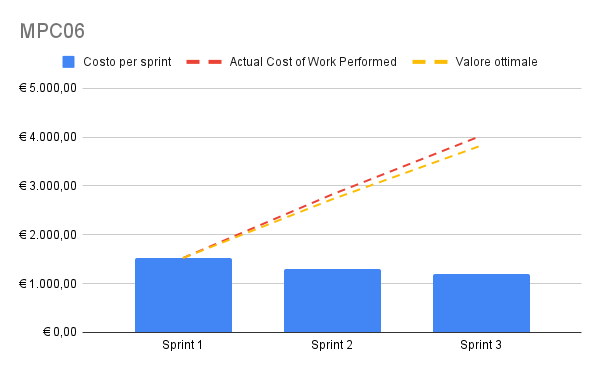
\includegraphics[width=0.7\textwidth]{img/MPC06.png}
    \caption{MPC06 - Actual Cost of Work Performed}
    \label{fig:mpc06}
\end{figure}

\newpage
\subsection{MPD1 - Indice di Gulpease}
\label{s:mpd1}
Il grafico in Figura \ref{fig:mpd1} mostra un miglioramento nella leggibilità media dei documenti redatti, avvenuto a seguito della fase di Candidatura.\\
Questo miglioramento è dovuto alla definizione di metriche di qualità che hanno portato il gruppo a prestare maggiore attenzione durante la scrittura della documentazione.
Il valore medio dell'indice di Gulpease ha così superato, per la fase RTB, la soglia di accettabilità.

\begin{figure}[htbp]
    \centering
    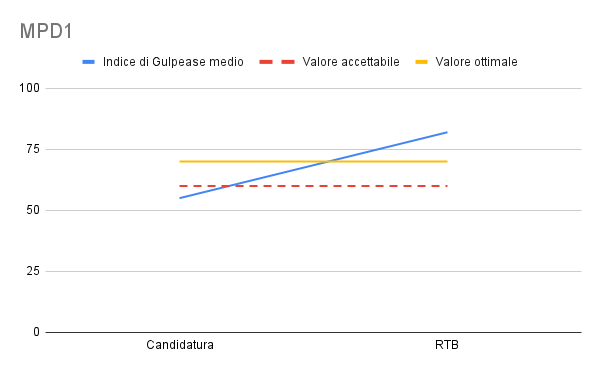
\includegraphics[width=0.7\textwidth]{img/MPD1.png}
    \caption{MPD1 - Indice di Gulpease}
    \label{fig:mpd1}
\end{figure}